
%(BEGIN_QUESTION)
% Copyright 2010, Tony R. Kuphaldt, released under the Creative Commons Attribution License (v 1.0)
% This means you may do almost anything with this work of mine, so long as you give me proper credit

Suppose we have a Koyo ``CLICK'' PLC connected to three momentary-contact pushbutton switches as shown in this illustration:

$$\includegraphics[width=15.5cm]{i04638x01.eps}$$

Determine the necessary switch actuation statuses (i.e. pressed versus unpressed) to turn the lamp on given the following program running in the PLC:

$$\includegraphics[width=15.5cm]{i04638x02.eps}$$

\vskip 20pt \vbox{\hrule \hbox{\strut \vrule{} {\bf Suggestions for Socratic discussion} \vrule} \hrule}

\begin{itemize}
\item{} Identify the significance of the labels ``X'' and ``Y'' for this PLC's bits.  What do you suppose ``X'' signifies?  What do you suppose ``Y'' signifies?
\end{itemize}

\underbar{file i04638}
%(END_QUESTION)





%(BEGIN_ANSWER)

In order for the lamp to energize, virtual coil {\tt Y1} must be colored.  In order to color this coil instruction, virtual contact {\tt X3} must be colored, and either virtual contacts {\tt X1} or {\it X2} must be colored.  Since the {\tt X3} contact is NO and both {\tt X1} and {\tt X2} contacts are NC, this requires input {\tt X3} to be powered, and either input {\tt X1} or {\tt X2} to be unpowered.

\vskip 10pt

Thus, NO pushbutton ``C'' must be pressed, and either NO pushbutton ``A'' released or NC pushbutton ``B'' pressed:

\begin{itemize}
\item{} Switch A = {\bf released} {\it or} Switch B = {\bf pressed}
\item{} Switch C = {\bf pressed}
\end{itemize}

%(END_ANSWER)





%(BEGIN_NOTES)


%INDEX% PLC, relating I/O status to virtual elements 

%(END_NOTES)


